\documentclass{article}[12pt]
\usepackage{listings}
\usepackage{color}
\usepackage{amsmath}
\usepackage{graphicx}
\usepackage{float}
\usepackage{amssymb}
\usepackage{mathtools,amssymb}
\usepackage{amsfonts}
\usepackage{amsthm}
\usepackage[linguistics]{forest}
\usepackage[utf8]{inputenc} 
\usepackage{chngcntr}
\usepackage{subcaption}
\usepackage[top=2in, bottom=1.5in, left=1in, right=1in]{geometry}
\usepackage{graphicx}
\usepackage{amsfonts}
\usepackage{amssymb}
\usepackage{amsmath}
\usepackage{setspace}
\setstretch{1,4}

\usetikzlibrary{quotes,arrows.meta}
\tikzset{
  annotated cuboid/.pic={
    \tikzset{%
      every edge quotes/.append style={midway, auto},
      /cuboid/.cd,
      #1
    }
    \draw [every edge/.append style={pic actions, densely dashed, opacity=0.5}, pic actions]
    (0,0,0) coordinate (o) -- ++(-\cubescale*\cubex,0,0) coordinate (a) -- ++(0,-\cubescale*\cubey,0) coordinate (b) edge coordinate [pos=1] (g) ++(0,0,-\cubescale*\cubez)  -- ++(\cubescale*\cubex,0,0) coordinate (c) -- cycle
    (o) -- ++(0,0,-\cubescale*\cubez) coordinate (d) -- ++(0,-\cubescale*\cubey,0) coordinate (e) edge (g) -- (c) -- cycle
    (o) -- (a) -- ++(0,0,-\cubescale*\cubez) coordinate (f) edge (g) -- (d) -- cycle;
    \path [every edge/.append style={pic actions, |-|}]
    (b) +(0,-5pt) coordinate (b1) edge ["\cubex \cubeunits"'] (b1 -| c)
    (b) +(-5pt,0) coordinate (b2) edge ["\cubey \cubeunits"] (b2 |- a)
    (c) +(3.5pt,-3.5pt) coordinate (c2) edge ["\cubez \cubeunits"'] ([xshift=3.5pt,yshift=-3.5pt]e)
    ;
  },
  /cuboid/.search also={/tikz},
  /cuboid/.cd,
  width/.store in=\cubex,
  height/.store in=\cubey,
  depth/.store in=\cubez,
  units/.store in=\cubeunits,
  scale/.store in=\cubescale,
  width=10,
  height=10,
  depth=10,
  units=cm,
  scale=.1,
}






\newcommand{\R}{\mathbb{R}}

\newcommand{\change}{\textcolor{blue}}
\newcommand{\argmin}{\mathop{\mathrm{arg\,min}}}
\newcommand{\argmax}{\mathop{\mathrm{arg\,max}}} 

\counterwithin*{section}{part}
\definecolor{mGreen}{rgb}{0,0.6,0}
\definecolor{mGray}{rgb}{0.5,0.5,0.5}
\definecolor{mPurple}{rgb}{0.58,0,0.82}
\definecolor{backgroundColour}{rgb}{0.95,0.95,0.92}
\lstdefinestyle{CStyle}{
    backgroundcolor=\color{backgroundColour},   
    commentstyle=\color{mGreen},
    keywordstyle=\color{magenta},
    numberstyle=\tiny\color{mGray},
    stringstyle=\color{mPurple},
    basicstyle=\footnotesize,
    breakatwhitespace=false,         
    breaklines=true,                 
    captionpos=b,                    
    keepspaces=true,                 
    numbers=left,                    
    numbersep=5pt,                  
    showspaces=false,                
    showstringspaces=false,
    showtabs=false,                  
    tabsize=2,
    language=C
}

\title{PLDAC - Etude de différentes techniques pour la classification de signaux d'EEG et MEG}
\author{Buton Nicolas}
\renewcommand{\contentsname}{Table des matières}
\begin{document}
\pagenumbering{gobble}
\maketitle
\begin{center}

\includegraphics[scale=1]{images/logoSorbonne.jpg}
\end{center}
\newpage
\tableofcontents
\newpage
\pagenumbering{arabic}
\part{Introduction}
Les signaux étudié seront des signaux d'Électroencéphalographie(EEG) et de Magnétoencéphalographie(MEG). Le premier consiste a enregistrer les signaux électrique a la surface du crane grâce a des électrodes, le second enregistre l'activité magnétique induite par l'activité des neurones grâce a un ensemble de magnétomètre.Notre étude ce place dans le cadre de l'analyse de série temporelle multivarié. On retrouve ces séries dans plusieurs domaine comme en finance, géophysique et dans notre cas dans les BCI(Brain Computer Interface). Chaque variable possède une dimension temporel et de plus chaque variable est lié au niveau spatial aux autres.\\

Une des premières difficulté des interfaces cerveaux machines c'est qu'elle ont besoin de réagir vite et donc on doit analyser le signal sur un laps de temps court, ce qui nous donne peut de données pour voir les liens entre les différentes variables. Une autres difficultés pour traiter ces signaux est le fait que les électrodes ne sont jamais situées exactement au même endroit sur le crane entre chaque essai, et entre chaque personne. De plus il peut y avoir beaucoup de bruit généré par le matériel ou les mouvement de l'utilisateur par exemple.\\

Historiquement la classification sur de tels signaux ce faisait avec des méthodes linéaire, par exemple avec des SVM, regression logistique. Cela avait des performances assez faible et il fallait donc répéter l’expérience plusieurs fois. Par la suite Alexandre Barachant à proposé d'utilisé les méthodes riemanniennes, celle ci permette de prendre en compte la spatialité de données et sont plus robuste. Cette robustesse vient du fait que la géométrie de Riemann permet de manipuler des matrice de covariance, car on peut définir une distance entre matrice symetrique définit positive, et les matrices de covariance font partie de ce groupe. Ces méthodes ont permit d'attaquer des taches plus compliqué comme le transfert entre sujet. On entraîne notre modèle en utilisant un sujet et par la suite on peut faire des prédiction sur un autre sujet.\\

C'est pour cela qu'aujourd'hui dans les méthodes de l’état de l'art utilise encore la géométrie riemannienne. Par la suite nous allons comparer ces méthodes avec de la géométrie riemannienne avec d'autres méthodes plus classique mais par forcément toute exploré, ainsi qu'une méthode de deep learning(un réseaux convolutionel). Nous essayerons plusieurs combinaison avec des méthodes d'annalyse de signal comme la transformer de fourier, des filtres et aussi d'autre façon de traiter les matrices de covariance, ainsi que des modeles comme des SVM et KNN.\\

On pourra voir que pour des cas simple comme l'ouverture et la fermeture des yeux qui possede un singal trés fort sur un EEG on a deja de trés bon resultat avec des méthodes simple, f1-score de 0.77 sur la classe minoriataire avec une transformer de fourier puis un SVM et une taille de fenettre adapté(détaillé dans la partie expériementation), et avec un Minimum distance to Mean et de la geometrie riemannienne on obtient un F1-score de 0.84.\\

Ps : Chanel et canaux seront utilisé de façon interchangeable dans la suite de ce document.
\part{État de l'art - la géometrie de riemann}
\section{Distance}
Les matrices de covariance sont des matrices symétrique et définit positive.
Pour deux matrice $\mathbf{\Sigma}_1$ et $\mathbf{\Sigma}_2$ leurs distances est d’après la géométrie de Riemann est la suivante :\\
\begin{equation}
\label{eq:Rgeodistance}
\delta_R(\mathbf{\Sigma}_1,\mathbf{\Sigma}_2) 
= 
\Vert \mathrm{log} \left( \mathbf{\Sigma}_1^{-1/2} \mathbf{\Sigma}_2 \mathbf{\Sigma}_1^{-1/2} \right) \Vert_F
=
\left[ \sum_{c=1}^{C} \log^2 \lambda_c \right]^{1/2},
\end{equation}
où $\lambda_c, c=1\ldots C$ sont les valeurs propres réelles de $\mathbf{\Sigma}_1^{-1/2} \mathbf{\Sigma}_2 \mathbf{\Sigma}_1^{-1/2}$ et C le nombre d’électrodes.
\\
F :Norme de Frobenius

\section{Moyenne géometrique}
Pour définir la matrice moyenne nous ne possédons pas d'expression explicite.
Fréchet mean
\begin{equation}
\mathfrak{G} \left( \mathbf{\Sigma}_1,\ldots,\mathbf{\Sigma}_I \right) = \argmin_{\mathbf{\Sigma}} 
\sum_{i=1}^{I} 
\delta_R^2 \left( \mathbf{\Sigma},\mathbf{\Sigma}_i \right).
\label{eq:geo_mean}
\end{equation}
Pour la calculer on peut utiliser une descente de gradient.

\section{Espace tangent}
On peut projeter un point de l'espace de Riemann définit par une matrice NxN sur un espace tangent avec N(N+1)/2 dimensions. Cet espace tangent est un espace euclidien. On peut approximer des distances de l'espace de Riemann par des distance dans l'espace tangent et cela fonctionne assez bien localement.
\begin{figure}[H]
\begin{center}
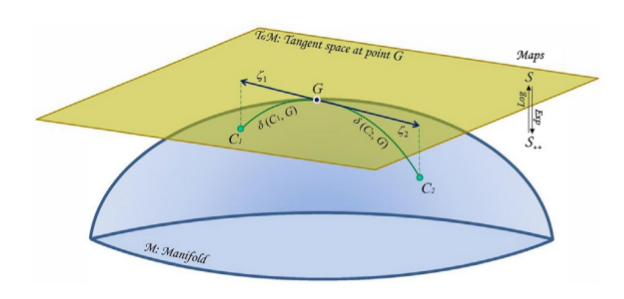
\includegraphics[scale=0.5]{images/Riemann_tangent_space.png}
\end{center}
\caption{Affichage del'espace tangent}
\end{figure}
Article sur la géométrie de Riemann : \\
- Brain invader \cite{congedo_brain_nodate} \\
- Geometrie de riemann \cite{congedo_riemannian_2017}\\


\part{Les différents modèles}
\section{Arbre des modèles}
Nous allons représenter a l'aide d'un arbre les différentes méthodes que nous allons tester par la suite.
\begin{center}
\begin{forest}
[Signal brut
  [Filtre passe-bas
	[SVM(8)]  
	[KNN(9)]
  ]
  [TF
  	[SVM(1)]
  	[KNN(2)]
  ]
  [Cov
  	[SVM(3)]
  	[MDM(4)]
  	[KNN(5)]
  ]
  [SVM(6)]
  [KNN(7)]
  [CTR(8)]
]
\end{forest}
\end{center}

Légende :\\
Cov : Matrice de covariance\\
TF : Transformé de fourier\\
MDM : Minimum Distance to Mean\\
CTR : Chaine de traitement riemannienne, détaillé plus loin.
\\

\section{Format des données}
En entrée deux format sont possible. Le premier est une serie temporel pour chaque éléctrodes ainssi que les labels pour chaque données d'entrée.\\
Notons :\\
C : le nombre de canaux.\\
T : le temps écoulé en seconde pendant l'enregistrement des données.\\
f : la fréquence d’échantillonnage du signal.\\
TT : le temps d'un trial.\\
NT : le nombre de trial.\\
Nous dispossons donc d'une matrice de taille Cx(T*f), ainsi que d'un vecteur de label de taille (T*f).\\
Mais un deuxieme format d'entrée est possible, en découpant par trial, a chaque trial correspond un label.\\

Nous disposons donc d'un tenseur de taille (TT*f)xCxNT, et d'un vecteur de label de taille NT.\\
On peut passer du premier formalisme a l'autre en découpant par trial(en définissant une taille de fenêtre) mais nous avons plusieurs possibilité pour savoir quels labels associé a ce trial (label majoritaire,premier label,dernier label,etc...).\\
\section{Description des modèles}
\subsection{1 et 2 - SVM et KNN avec une transformer de fourrier}
La première étape de notre modèle est d'effectuer une transformer de fourrier, c'est a dire passé d'un signal temporel à un signal fréquentiel. Pour calculer nous utiliserons l'algorithme FFT(Fast fourier transform).Nous garderons uniquement le modules pour rester avec des valeurs réelles plutôt que complexe.\\

Ensuite nous utilisons un SVM pour prédire les labels dans un cas et un KNN dans l'autre.
\subsection{3,4 et 5 - SVM,MDM et KNN avec matrice de covariance }
Pour cette approche nous devons passer au deuxième format de données(décrit dans la partie précédente), si les données nous sont donné dans le premier format nous devons définir une taille de fenêtre et une méthode d'attribution des labels.\\
Ensuite on calcul la matrice de covariance :\\
$
\mathbf{\Sigma}_{i}=\frac{1}{C} \tilde{\mathbf{X}} \overline{\mathbf{X}}^{T}
$
Avec X ma matrice d'entrée.
\subsection{6 et 7 - SVM et KNN sur les données brut}
Cette approche est la plus simple et on utilise simplement un vecteur de la taille le nombre de capteur, c'est à dire un relevé a un instant t des capteurs pour prédire un labels.
\subsection{8 et 9 - SVM et KNN avec un filtre passe bas}
Nous définissons un filtre passe bas avec la moyenne sur un fennettre glissante. Donc nous avons deux paramettre le premier est la longueur de la fennetre, sur combien on moyenne et le deuxieme est le decallage de cette fennettre. On peut mettre la longueur de la fennettre egale au decalage si on ne veux pas de chevauchement.
\subsection{8 - Chaine de traitement riemannienne}
Par la suite je vais décrire la chaine de traitement etape par etape.\\
1 - On garde uniquement 1 secondes sur les 1.5 secondes de signal car le stimulus intervient qu’après 0.5 secondes. \\
2 - On filtre le signal avec un filtre passe bande de Butterworth d'ordre 5 entre 1Hz et 20Hz.\\
3 - Par la suite on effectue un filtrage spatial, on extrait K canaux virtuel par classe.\\
On commence par définir la moyenne sur chaque classe :
$$ \mbox{\Large $ 
\mathbf{P}^{(k)}=\frac{1}{ | \mathcal{I}^{(k) |}} \sum_{i \in \mathcal{I}^{(k)}} \mathbf{X}_{i_{1}}
$ } $$
Ensuite notre but est d'optimiser les W par descente de gradient. En maximisant cette fonction :
$$ \mbox{\Large $ 
\mathbf{w}^{*}=\underset{\mathbf{w}}{\arg \max } \frac{\mathbf{w}^{T} \mathbf{P}^{(k)} \mathbf{P}^{(k) T} \mathbf{w}}{\mathbf{w}^{T} \mathbf{X} \mathbf{X}^{T} \mathbf{w}}
$ } $$
On introduit les Zi.
$$ \mbox{\Large $ 
\mathbf{Z}_{i}=\mathbf{W}^{T} \mathbf{X}_{i}
$ } $$
Cela nous permet de définir de nouvelles carasctéristique, donc a chaque Xi d'entrée sur C canaux on le projette sur K canaux.
$$ \mbox{\Large $ 
\tilde{\boldsymbol{Z}}_{i}=\left[ \begin{array}{c}{\mathbf{W}^{(0)^{T}} \mathbf{P}^{(0)}} \\ {\mathbf{W}^{(1)^{T}} \mathbf{P}^{(1)}} \\ {\mathbf{Z}_{i}}\end{array}\right]
$ } $$
Et l'on calcul la covariance de cette nouvelle matrice de caractéristique.
$$ \mbox{\Large $ 
\boldsymbol{\Sigma}_{i}=\frac{1}{N} \tilde{\mathbf{Z}}_{i} \tilde{\mathbf{Z}}_{i}^{T}
$ } $$

4 - On définit une nouvelle entrée comme étant la concaténation :\\
- du signal moyen de la classe 1 auquel on multiple par W0 pour les projeter sur les channels virtuelles appris précédemment.\\
- idem pour la classe 2\\
- Et ensuite le signal Xi projeter sur les 8 channels.\\
5 - On calcul la covariance de cette matrice.\\
6 - On projette cette matrice sur l'espace tangent.\\
7 - On estime pour les 15 autre sujets avec ce filtre spatial
8 - On fait la même chose pour les 15 autres sujet et on concaténe.\\
9 - Régression logistique avec une régularisation lasso.\\
Les figures suivantes représentes la forme des matrices au fur et a mesure du processus. Elles sont a lire de gauche a droite et de haut en bas.
\\
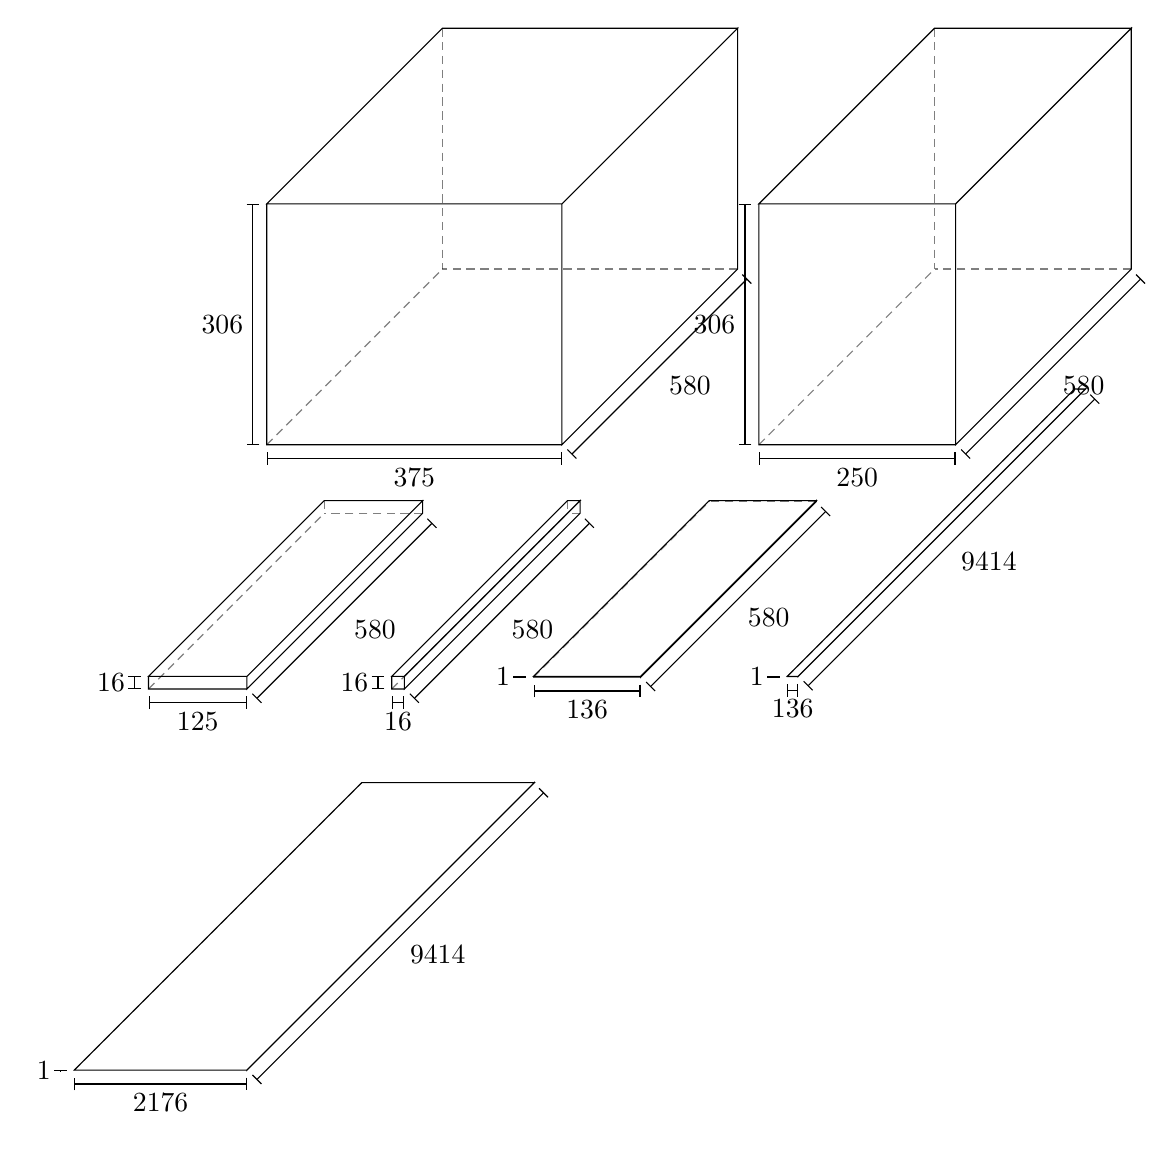
\begin{tikzpicture}
  \pic at (0,10) {annotated cuboid={width=375, height=306, depth=580, scale=.01, units=}};
  \pic at (5,10) {annotated cuboid={width=250, height=306, depth=580, scale=.01, units=}};
   \pic at (-4,4) {annotated cuboid={width=125, height=16, depth=580, scale=.01, units=}};
   \pic at (-2,4) {annotated cuboid={width=16, height=16, depth=580, scale=.01, units=}};
   \pic at (1,4) {annotated cuboid={width=136, height=1, depth=580, scale=.01, units=}};
   \pic at (3,4) {annotated cuboid={width=136, height=1, depth=9414, scale=.001, units=}};
   \pic at (-4,-1) {annotated cuboid={width=2176, height=1, depth=9414, scale=.001, units=}};
\end{tikzpicture}


\part{Experimentations}
Dans ce rapport nous étudierons nos méthodes sur 3 datasets différents : Eye close/eye open, brain invader et DecMeg2014.\\
Tout le code et les résulats correspondant aux expérience peuvent etre trouvés sur github. \footnote{https://github.com/rootNico/PLDAC}
\section{Prise en main sur un dataset simple}
\subsection{Decription du dataset eye close/eye open}
Ce dataset contient les données enregistré avec un casque EEG ou l'on a demandé au sujet d'ouvrir ou de fermer les yeux a certain moment. La tache a accomplir est de classifier a chaque enregistrement si la personne a les yeux ouvert ou fermé.\\
\\
Le signal est échantillonné à 512Hz. Il y a 7 femmes et 13 hommes pour un total de 20 participant pour ce dataset. L'age moyen est de 25.8 ans avec un écart type de 5.27 et une médiane a 25.5 ans. 18 sujets ont entre 19 et 28 ans et deux participants ont respectivement 33 ans et 44 ans.Le casque d'enregistrement est composé de 16 électrodes.\\
\\
On commence par visualiser le signal des 16 électrodes ainsi que leurs labels associé au cours du temps.\\
\begin{figure}[H]
\begin{center}
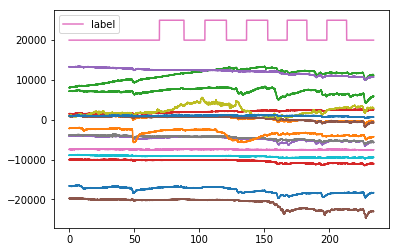
\includegraphics[scale=0.8]{images/donnees_entree.png}
\end{center}
\caption{Affichage des données brut}
\end{figure}

\subsection{Résultat des différents algorithmes}
Prédiction théorique : \\
La méthode 6 et 7 ne devrais pas fonctionner car avec une seule données c'est difficile de faire quoi que ce soit.\\
La méthode 8 et 9 ne devrais pas fonctionner car il n'y aura pas invariance par translation.\\

Toute les resulats suivant on été obtenu avec les données d'un seul sujet, avec une validation croisée en 5 parties.
\subsubsection{Valeurs de k pour KNN}

\begin{figure}[H]
\begin{center}
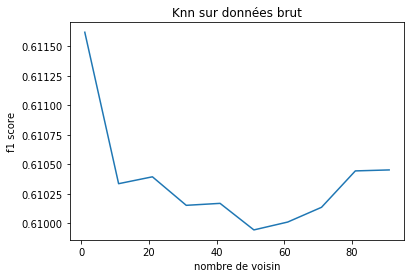
\includegraphics[scale=0.7]{images/f1_score_knn_brut.png}
\end{center}
\caption{F1 Score(en cross validation) du knn sur les données brute en fonction du nombre de voisin}
\end{figure}

On peut voir que la valeur de K=1 est meilleur.
\subsubsection{Études sur la longueur de la fenêtre optimale}
On remarque qu'avec des tailles de fennettre trés petite on a de trés bon résultat mais cela vient du fait qu'on utilise des algorithme tel que le KNN et le MDM qui 
\begin{figure*}
        \centering
        \begin{subfigure}[b]{0.475\textwidth}
            \centering
            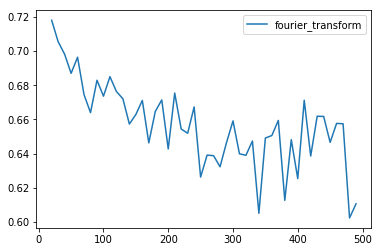
\includegraphics[width=\textwidth]{images/knn_tf_f1Score.png}
            \caption[Network2]%
            {{\small KNN transformée de fourier}}    
            \label{fig:mean and std of net14}
        \end{subfigure}
        \hfill
        \begin{subfigure}[b]{0.475\textwidth}  
            \centering 
            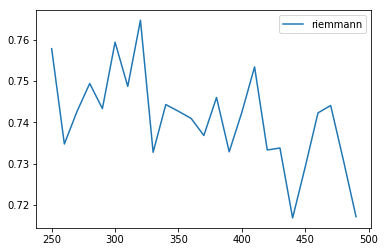
\includegraphics[width=\textwidth]{images/riemann_cov_knn_f1Score.png}
            \caption[]%
            {{\small Riemann Cov KNN }}    
            \label{fig:mean and std of net24}
        \end{subfigure}
        \vskip\baselineskip
        \begin{subfigure}[b]{0.475\textwidth}   
            \centering 
            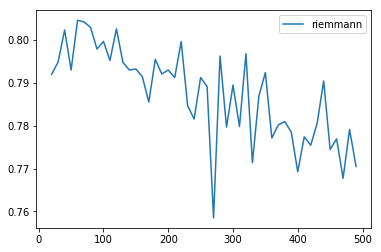
\includegraphics[width=\textwidth]{images/riemann_cov_MDM_f1Score.png}
            \caption[]%
            {{\small riemann MDM}}    
            \label{fig:mean and std of net34}
        \end{subfigure}
        \quad
        \begin{subfigure}[b]{0.475\textwidth}   
            \centering 
            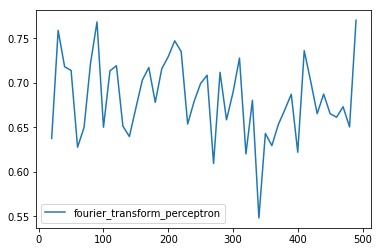
\includegraphics[width=\textwidth]{images/perceptron_tf_f1Score.png}
            \caption[]%
            {{\small SVM transformée de fourier }}    
            \label{fig:mean and std of net44}
        \end{subfigure}
        \caption[ F1 Score(en cross validation) en fonction du nombre de données par paquet]
        {\small F1 Score(en cross validation) en fonction du nombre de données par paquet} 
        \label{fig:mean and std of nets}
    \end{figure*}
    
\subsubsection{Tableau récapiltulatif}
f1-score arrondie à deux chiffre apres la virgule.\\
\begin{center}
\begin{tabular}{|l|c|}
  \hline
  Nom de l'algorithme & f1-score\\
  \hline
  SVM sur les données brut & 0.54 \\
  KNN sur les données brut & 0.61\\
  Riemann Cov MDM  & 0.84 \\
  Riemann Cov KNN & 0.77\\
  SVM filtre passe bas & 0.60 \\
  KNN filtre passe bas & 0.59 \\
  SVM transformée de fourier & 0.77 \\
  KNN transformée de fourier & 0.72 \\
  \hline
\end{tabular}
\end{center}
\section{Brain Invader}
\subsection{Description de la tache de machine learning}
Ce dataset à été enregistrer avec les sujets placer devant un pc ou une grille d'alien était représenté sur un écran.12 flashs dont 2 comprennent l'alien ciblé. Détecté les flash ou il y a l'alien en regardant l'activité cérébrale.Plusieurs tentative pour détruire l'alien.\\
Première tache : Classification binaire (le flash nous intéresse(il y a l'alien cible dedans) ou pas)\\
Deuxième tache : dans le groupe de 12 ou sont les deux flashs avec l'alien cible.\\

\begin{figure*}
        \centering
        \begin{subfigure}[b]{0.475\textwidth}
            \centering
            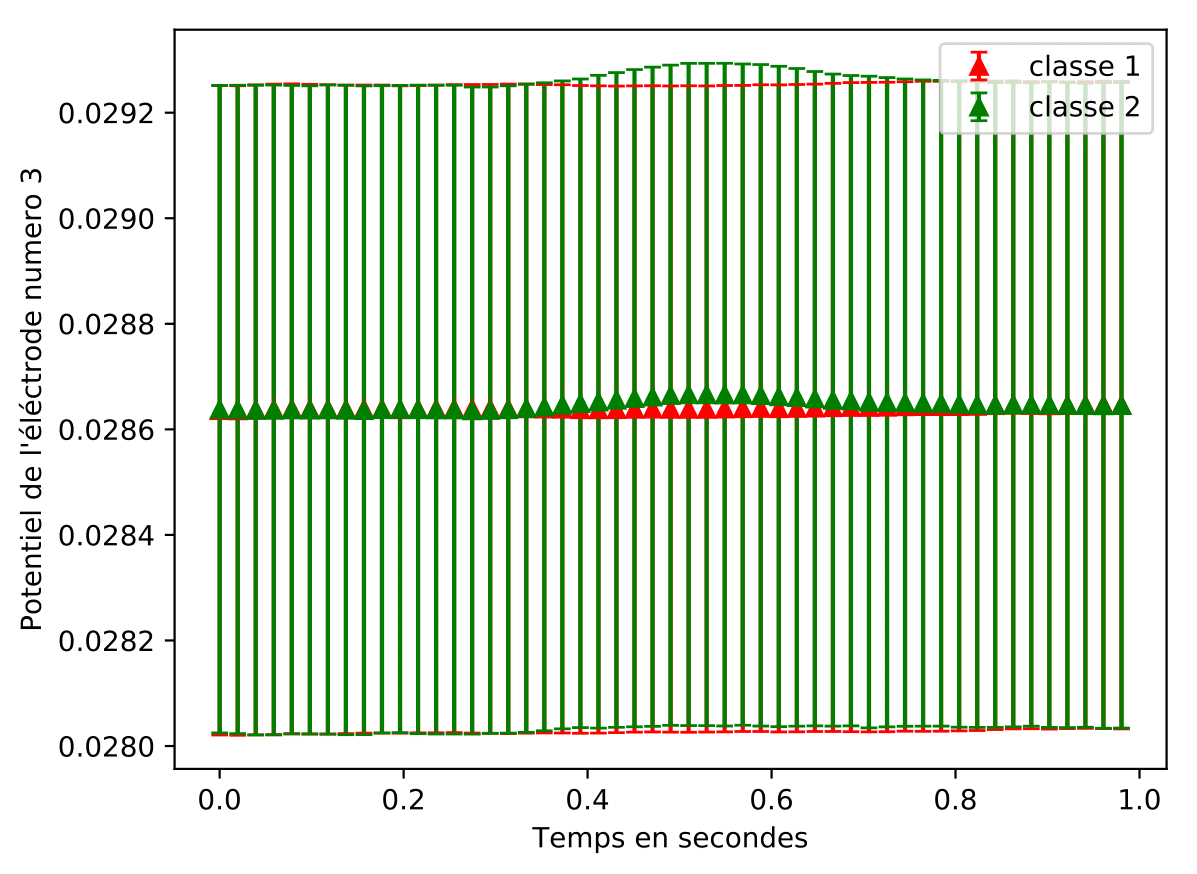
\includegraphics[width=\textwidth]{images/visuel_classe_mean_std-1.png}
            \caption[Network2]%
            {{\small visuel classe mean std}}    
            \label{fig:mean and std of net14}
        \end{subfigure}
        \hfill
        \begin{subfigure}[b]{0.475\textwidth}  
            \centering 
            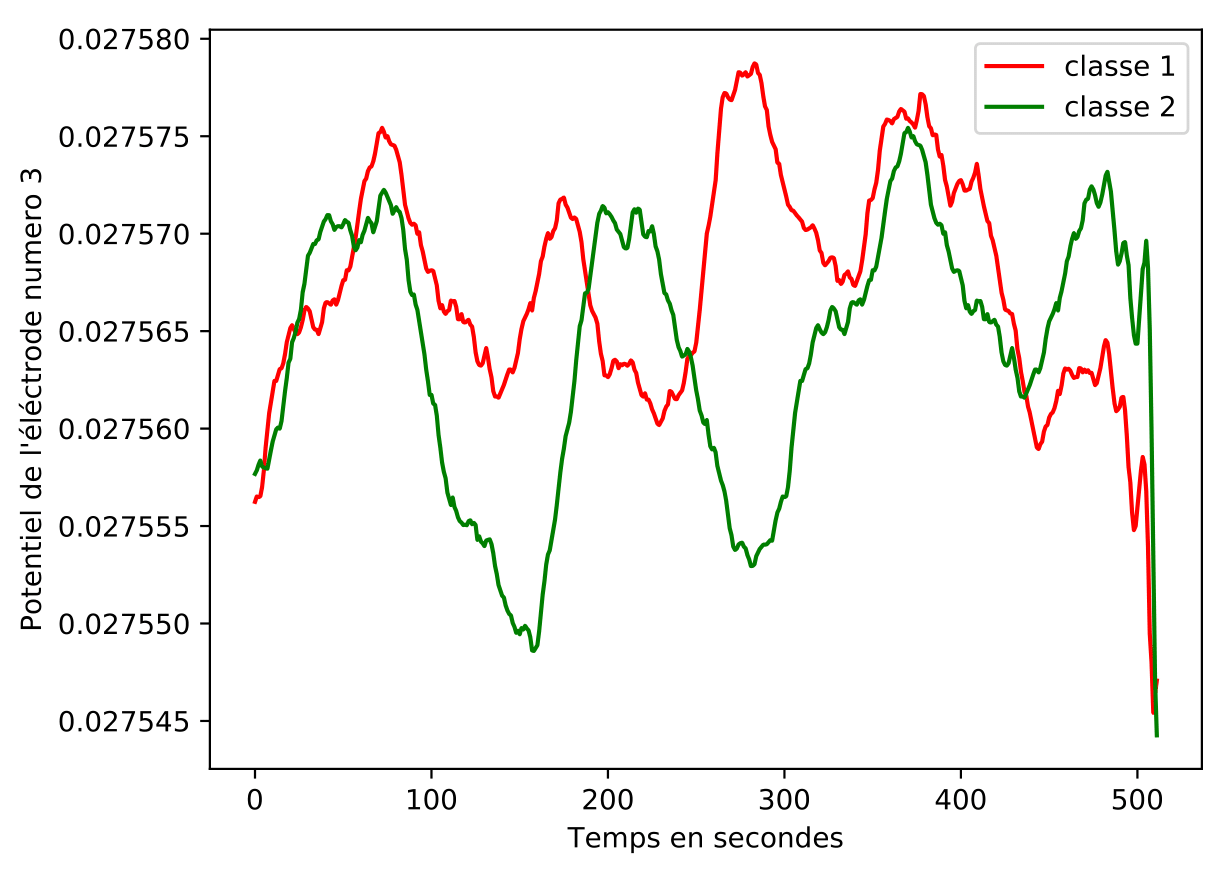
\includegraphics[width=\textwidth]{images/visuel_data_0-1.png}
            \caption[]%
            {{\small visuel data 0-1 }}    
            \label{fig:mean and std of net24}
        \end{subfigure}
        \caption[ Visualisation des classes]
        {\small Visualisation des classes} 
        \label{fig:mean and std of nets}
    \end{figure*}
    
F1-score des différents algorithme sur brain invader : \\
C'est resultat sont obtenu avec une cross validation sur tout les sujets mais en ne prenant en compte qu'un fichier par sujet pour une question de mémoire.
\begin{table}[]
\begin{tabular}{|l|l|l|l|l|}
\hline
nom de l'algorithme                                                              & 1 seconde         & 0,1 seconde       & 0,04 seconde      & moyenne           \\
\hline
passe bas KNN & 0,002487562189055 & 0,126738794435858 & 0,004889975550122 & 0,044705444058345 \\
knn tf & 0,019002375296912 & 0,029919447640967 & 0,124804992199688 & 0,057908938379189 \\
knn brut            & 0,071287128712871 & 0,104810996563574 & 0,027681660899654 & 0,067926595392033 \\
SVM brut       & 0,181818181818182 & 0                 & 0,214285714285714 & 0,132034632034632 \\
cov SVM & 0                 & 0,181818181818182 & 0,235294117647059 & 0,13903743315508  \\
SVM tf & 0,125             & 0,125             & 0,181818181818182 & 0,143939393939394 \\
passe bas SVM & 0,214285714285714 & 0,214285714285714 & 0,235294117647059 & 0,221288515406162 \\
riemann MDM     & 0,269889224572004 & 0,256206554121152 & 0,249661705006766 & 0,258585827899974\\
\hline
\end{tabular}
\end{table}

Comme on peut le voir tout les algorithme de sont pas présent, certain etait trop long a faire tournée et d'autre n'avais pas encore été introduit et le seront pour le dataset DecMeg2014 qui suit.\\

Aucun pré traitement n'a été fait sur le signal pour la géometrie de riemann et cela change beaucoup les resultats juste un filtre passe bande peut amélioré les resultats comme on va le voir par la suite. C'est aussi pour cela qu'on retrouve un SVM en deuxieme position.\\

Il n'a pas été possible de comparer les résultats avec les résultats de l'auteur du dataset car il manquait la composition des groupe d'alien qui clignotait.\\
\section{DecMeg2014}
\subsection{Description du dataset}
La tache que l'on doit réaliser avec le dataset DecMeg2014 est une classification binaire. Le but est de déterminer si le stimulus visuel est un visage clair ou un brouiller qui est montré au participant.L'activité de leurs cerveaux est enregistrer grâce à un appareil de magnetoencéphalographie. Cet appareil dispose de 306 magnétomètres.
\\
Ce dataset est extrait d'une compétition kaggle du même nom.
\\
23 sujets on participé à ce test avec environ 580 trials par sujet. Nous disposons de 16 sujets avec leurs labels associé et 7 sujets ou nous avons uniquement les données.
\subsection{Méthode d'évaluation}
Sur le dernier dataset DecMeg2014 nous disposons des données pour 16 sujets, nous procéderons donc comme décris ci-dessous pour l'évaluation de nos différentes méthodes :\\
Méthode 1 : entrainement sur une partie de 1 et eval sur 1 (validation croisée sur un seul)\\
Méthode 2 : entrainement sur 1 et évaluation sur tous les autres (16 expériences a faire)\\
Méthode 3 : entrainement sur 15 et évaluation sur 1 (16 expériences a faire )\\
Méthode 4 : entrainement sur 16 et eval sur 16 tout mélanger avec validation croisée.
\\
Ces façon d'évaluer nous permette de tester plusieurs caractéristique de nos modèles dont la capacité de transfert d'un sujet a l'autre.
\\
Pour chaque test on sauvegardera le f1 score sur la classe minoritaire.
\begin{table}[]
\begin{tabular}{|l|l|l|l|l|}
\hline
Nom de l’algorithme & Méthode 1         & Méthode 2           & Méthode 3          & Méthode 4          \\
\hline
CTR                 & 0,717 & 0.182 & 0.673 & 0.693 \\
conv1D              & 0,133         & 0.04                & 0.09               & 0.26               \\
passe bas SVM       & 0.0                & 0.0                   & 0.0                  & 0                  \\
riemann MDM         & 0,5524            & 0.12                & 0.43               & 0.49               \\
SVM brut            & 0.0                 & 0.0                   & 0                  & 0.0                  \\
SVM TF              & 0.0                 & 0.0                   & 0.0                  & 0.0      \\
\hline           
\end{tabular}
\end{table}
\part{Conclusion}
D'après nos résultat nous pouvons conclure que d'une part les pré traitement sur le signal sont trés important et que pour le moment avec des méthodes classique de deep learning on n'arrive pas a faire mieux qu'avec des méthodes riemanniennes. Il pourrais etre interessant de combiner des methodes de deep learning et de géometrie de riemann.
\bibliographystyle{ieeetr}
\bibliography{MyLibrary} 


\end{document}
